\section{Distributed crawler}\label{sec:distributed_crawler}

The distributed crawler forms the starting point of the system design.
It is responsible for fetching and processing web pages from the set of e-commerce websites and storing them in order to be processed in the later stages.
The crawler is designed to operate across multiple nodes, allowing it to scale horizontally and handle large volumes of data efficiently.
It also has built-in mechanisms for retries and exponential backoff to handle transient errors and avoid overwhelming the target websites with requests.

The crawler is implemented with the use of three subcomponents.
\begin{enumerate}
    \item \textbf{Crawler queue:} This is an Amazon SQS queue that holds the URLs to be crawled.
    It allows for decoupling the crawling process from the processing of the crawled data, enabling better scalability and fault tolerance.
    \item \textbf{Queue manager:} This is a lambda function which runs every 15 minutes, and is responsible for populating the crawler queue with new URLs to be crawled.
    \item \textbf{Crawler workers:} These are Amazon ECS tasks which loads URLs from the crawler queue, fetches the corresponding web pages, and saves their content.
\end{enumerate}

\subsection{Crawler queue}\label{subsec:crawler-queue}
The crawler queue is a fairly simple component.
It is implemented using Amazon SQS, which provides a reliable, scalable, and fully managed message queuing service.
The queue holds the URLs to be crawled, allowing the crawler workers to fetch and process them asynchronously.
This decoupling of the crawling process from the processing of the crawled data enables better scalability and fault tolerance.

It consists of two queues: a main queue and a dead-letter queue.
The main queue holds the URLs to be crawled, while the dead-letter queue holds the URLs that could not be processed successfully after a certain number of retries.
This allows for better error handling and monitoring of the crawling process, as failed URLs can be analyzed and reprocessed later.

The main queue is configured with a visibility timeout of 1 hour, which means that once a URL is fetched by a crawler worker, it will not be visible to other workers for 1 hour.
This allows the worker to have enough time to process the URL and avoid duplicate processing.
Once a URL is successfully processed, it is deleted from the queue, ensuring that it is not processed again.
Moreover, the main queue is configured with a maximum message retention period of 1 day, which means that if a URL is not processed within 1 day, it will be automatically deleted from the queue.
This prevents the queue from growing indefinitely and ensures that only relevant URLs are kept for processing.

\subsection{Queue manager}\label{subsec:queue-manager}
The queue manager is a lambda function that runs every 15 minutes and is responsible for populating the crawler queue with new URLs to be crawled.
It first checks whether the crawler queue is empty, and if it is not, it does nothing and exits.
If the queue is empty, it checks the database for any URLs which match at least one of the following criteria:
\begin{itemize}
    \item The URL has not been crawled even once.
    \item The URL is classified as a product page, but has not been crawled in the last 60 hours.
    \item The URL is classified as a non-product page, but has not been crawled in the last 7 days.
\end{itemize}
The queue manager fetches the URLs that match these criteria and adds them to the crawler queue for processing by the crawler workers.
This ensures that the crawler is continuously fetching and processing new data, while also re-crawling existing data to keep it up-to-date.
The figure~\ref{fig:crawler_queue_manager_logic} shows the logic of the queue manager in a flowchart format.

\begin{figure}[h]
    \centering
    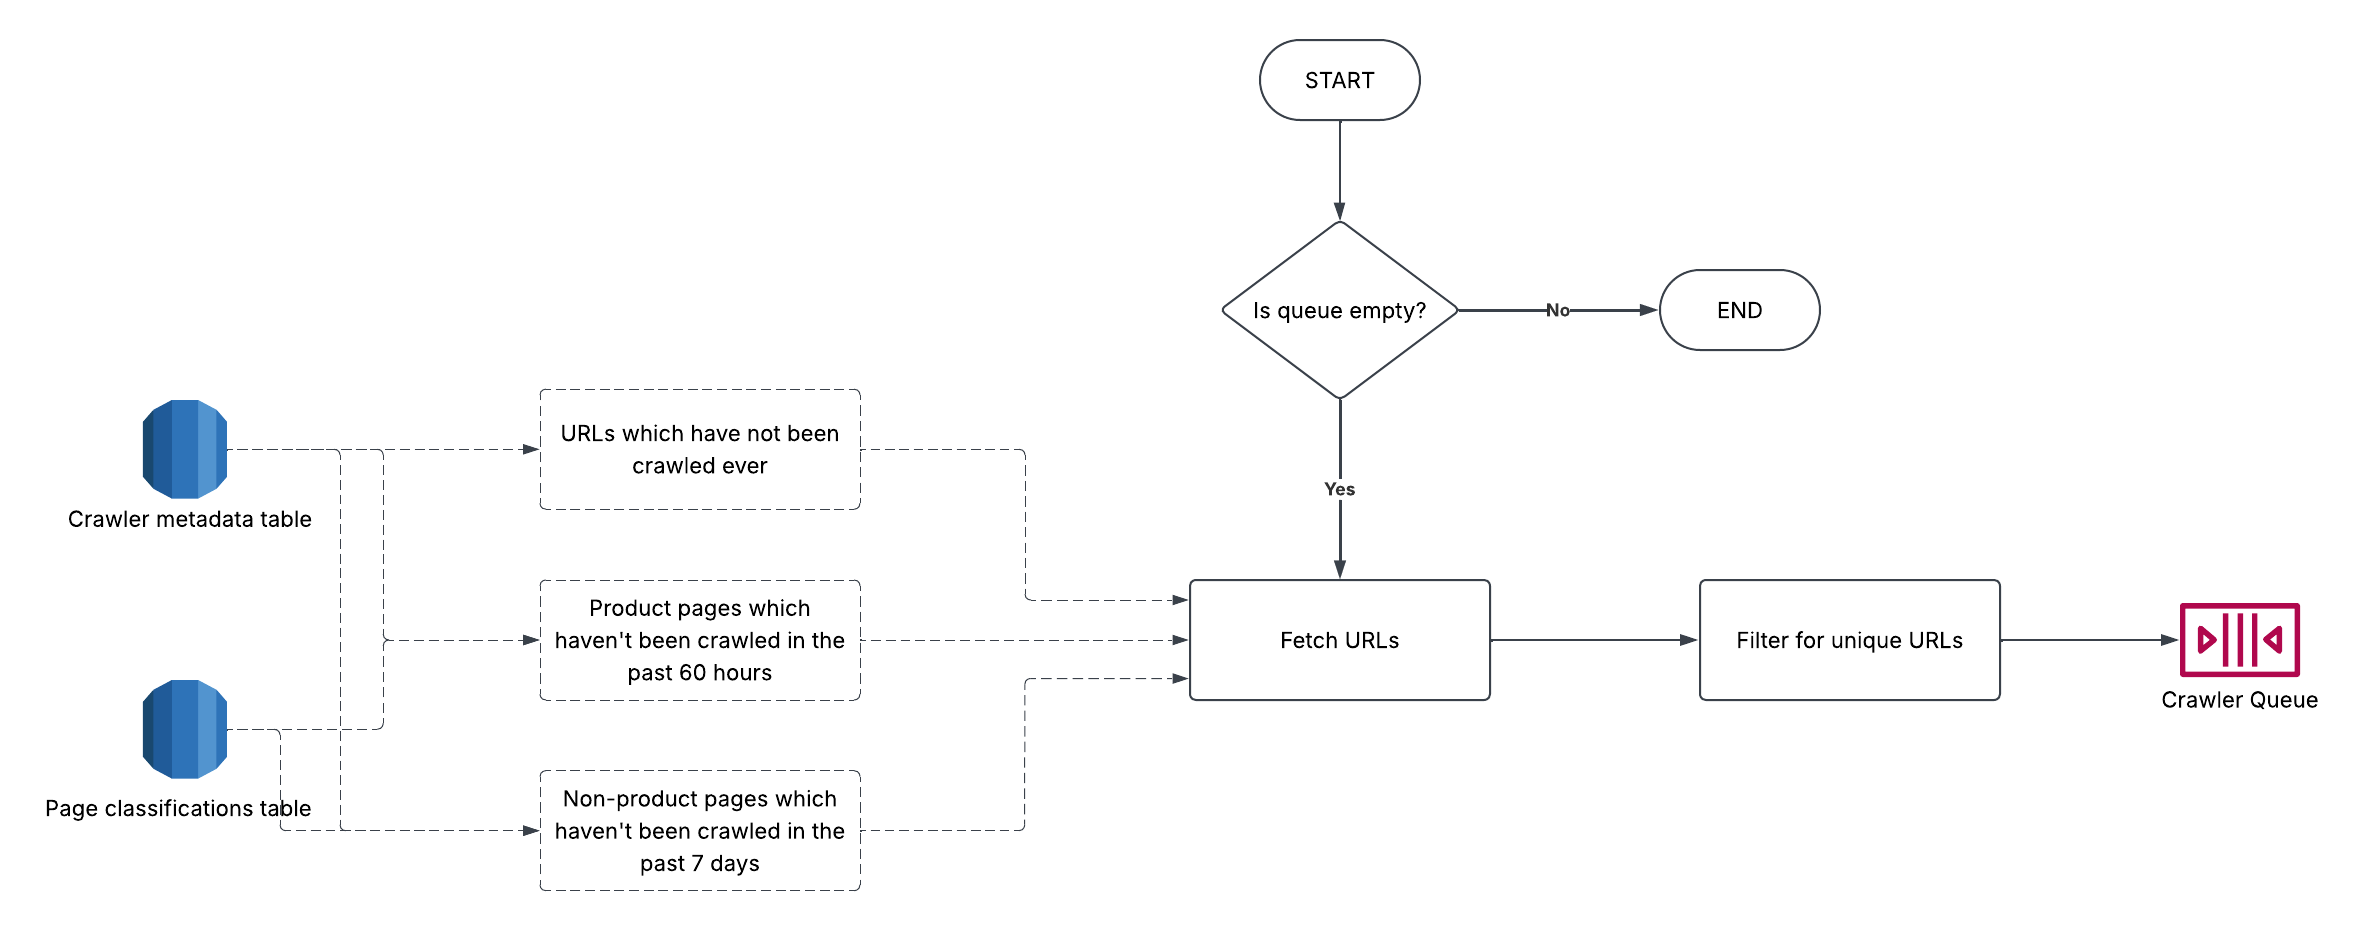
\includegraphics[width=\textwidth]{images/crawler_queue_manager_logic}~\caption{Crawler queue manager flow diagram}\label{fig:crawler_queue_manager_logic}
\end{figure}

The behaviour of the crawler ensures that each product page is crawled at least once every 3 days, while all other pages are crawled at roughly once every 7 days.

\subsection{Crawler workers}\label{subsec:crawler-workers}
The crawler workers are Amazon ECS tasks that are responsible for fetching and processing the web pages from the crawler queue.
Each worker loads a URL from the queue, fetches the corresponding web page, and saves its content to the database.
The workers are designed to operate in parallel, allowing for efficient processing of large volumes of data.
They also have built-in mechanisms for retries and exponential backoff to handle transient errors and avoid overwhelming the target websites with requests.

For most of the lifecycle of a processed page, the JavaScript library \texttt{Playwright} is used to interact with the page and retrieve its content.
Playwright is a powerful library that allows for automated browser interactions, enabling the crawler to handle dynamic content and JavaScript-heavy pages effectively.
It also supports pre-navigation and post-navigation hooks, which allow for custom logic to be executed before and after the page is loaded.
The figure~\ref{fig:crawler_worker_flowchart} presents the crawler worker logic as a flowchart.

For each URL fetched by a worker, the following actions are performed:
\begin{itemize}
    \item Checks if the URL belongs to an approved domain.
    If it does not, the URL is discarded and not processed further.
    \item The URL is compared against known blacklisted patterns, and if it matches any of them, it is discarded and not processed further.
    \item Checks the URL against the site's \texttt{robots.txt} file to ensure that the crawler is allowed to access the page.
    This is done to avoid crawling pages that are known to be irrelevant or problematic, such as login pages, checkout pages, malicious links, or pages that are known to cause issues with the crawler.
    \item Retrieves the initial content of the page using an HTTP GET request.
    \item Checks if the initial HTTP response is a redirect, and if so, follows the redirect to the final destination URL.
    \item Block the loading of images, external stylesheets, advertisements, and other non-essential resources via pre-navigation hooks to reduce bandwidth usage, minimize the load on the target servers, and speed up the crawling process.
    \item Waits up to 15 seconds for the page to load completely, including any dynamic content that may be generated by JavaScript.
    \item Downloads the final HTML content of the page and
        \subitem Saves it to an Amazon S3 bucket for further processing.
        \subitem Updates the crawler metadata table in the database with the status of the crawl and the last crawled timestamp.
    \item Checks whether the page contains any JSON-LD structured data, and if so,
        \subitem Check whether the page is a product page based on the JSON-LD data, and updates the page classification table in the database accordingly.
        \subitem Extracts the relevant product information from the JSON-LD data and saves it to the product information tables in the database.
    \item Detects all the outgoing hyperlinks on the page and adds them to crawler metadata table in the database for future crawling.
    \item Removes URL from the crawler queue to ensure that it is not processed again.
\end{itemize}

\begin{figure}[h]
    \centering
    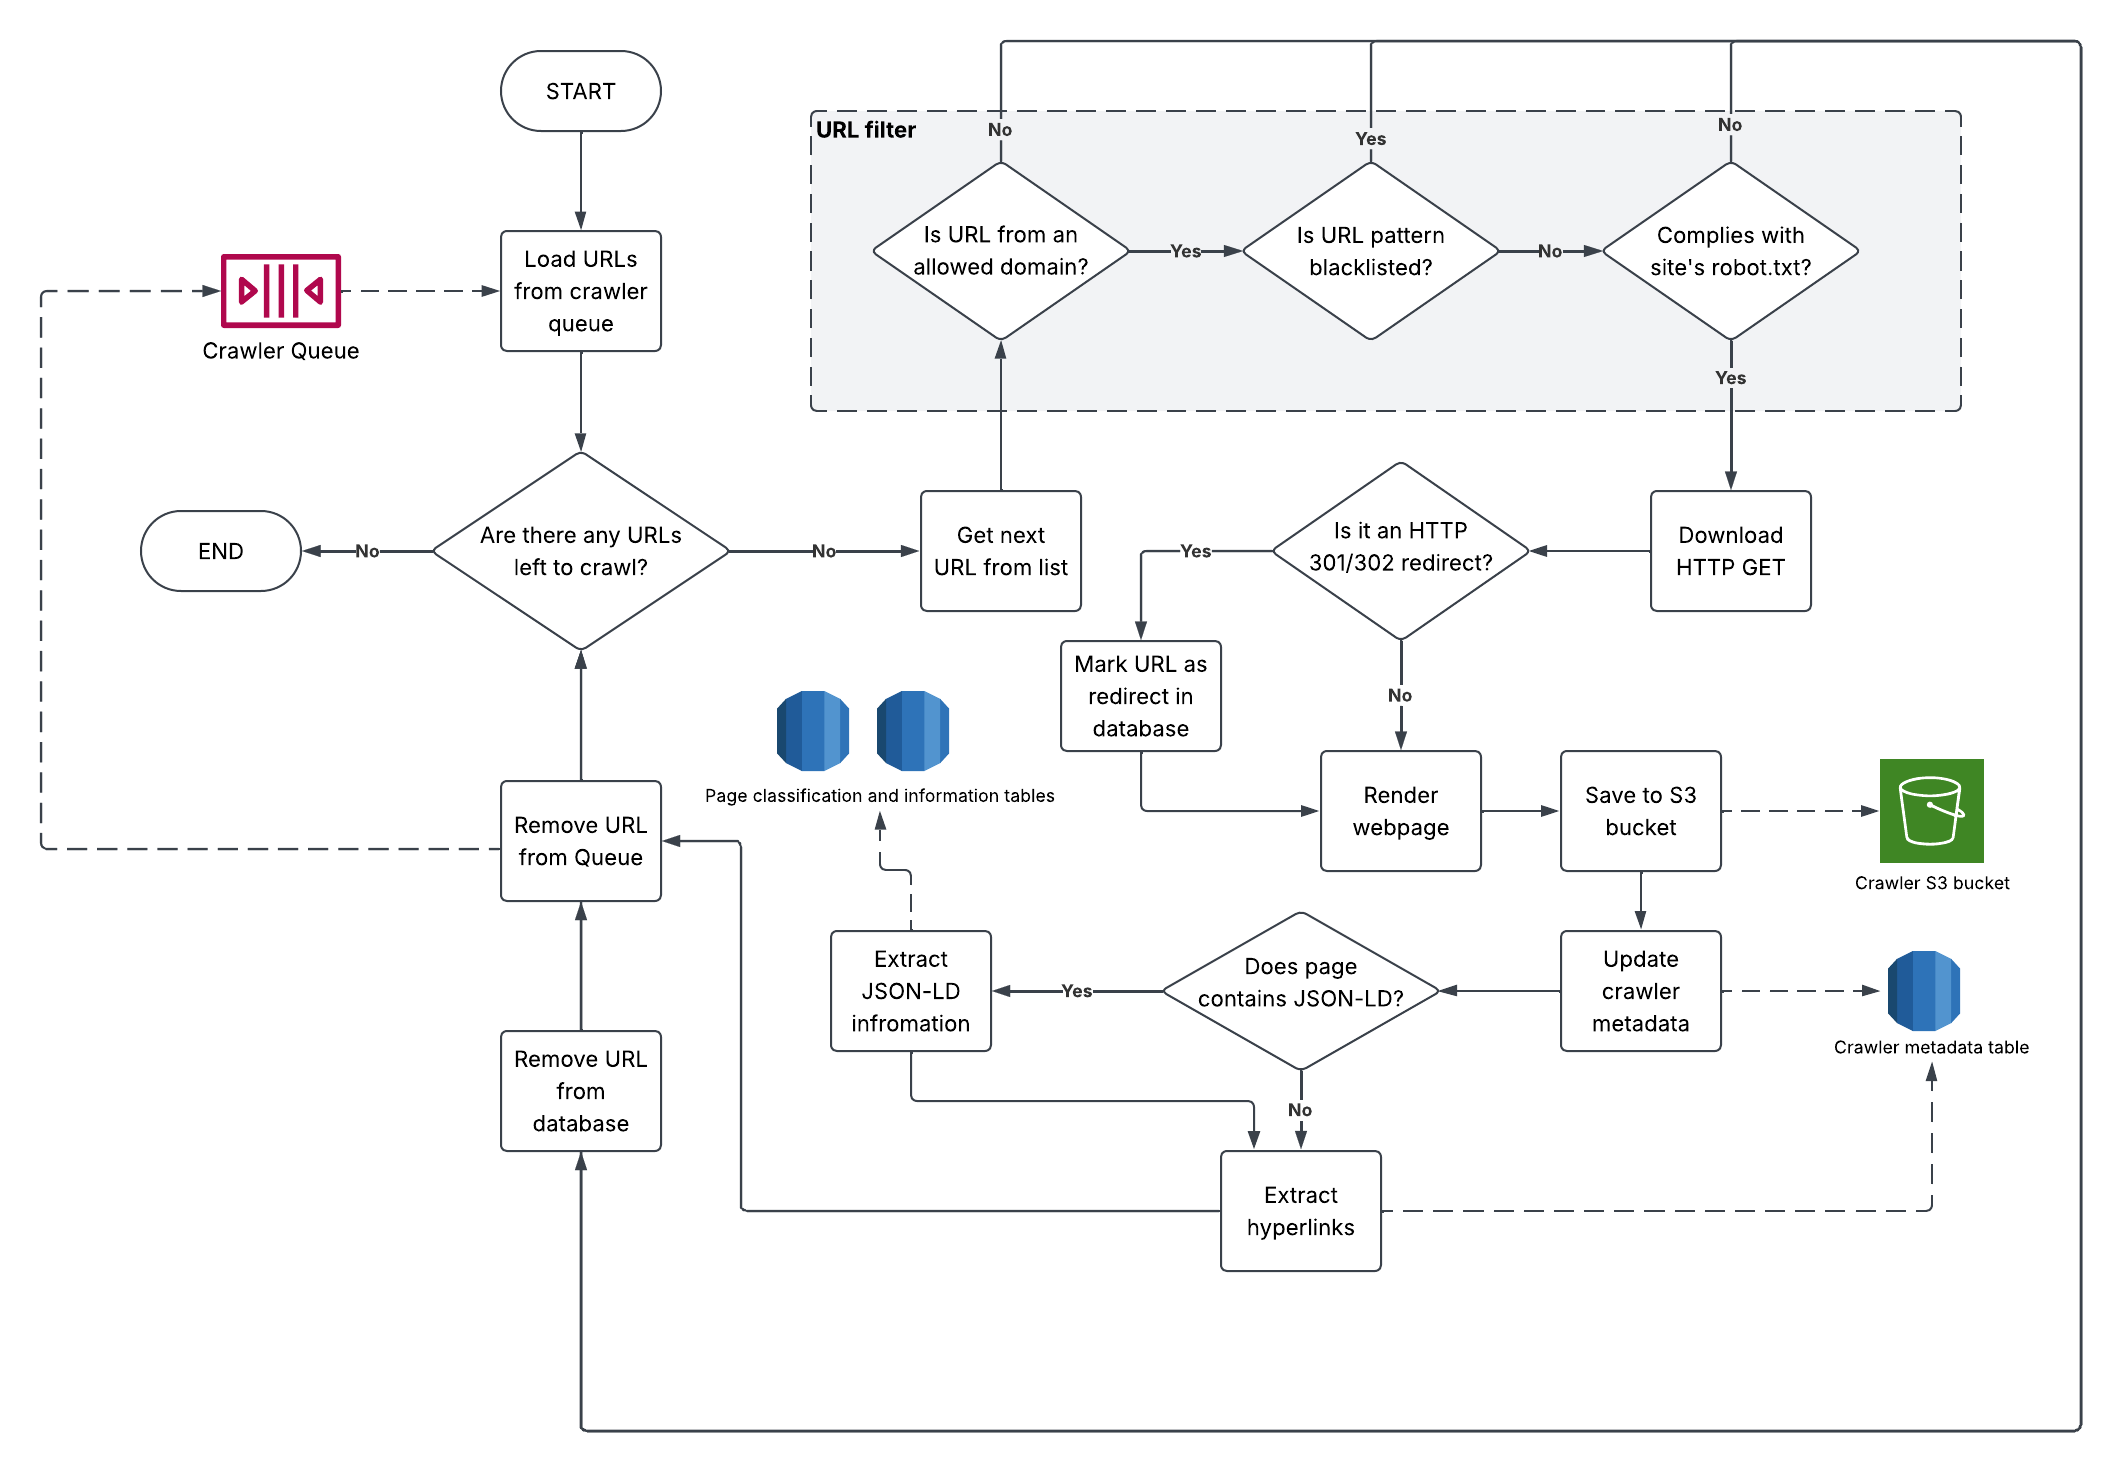
\includegraphics[width=\textwidth]{images/crawler_worker_flowchart}~\caption{Crawler worker flowchart}\label{fig:crawler_worker_flowchart}
\end{figure}

The crawler workers are run as tasks on AWS Fargate Spot, which allows for cost-effective and scalable execution of containerized applications.
However since they are run on spot instances, they can be interrupted at any time by AWS.
To handle this, the crawler workers are designed to be stateless and idempotent, meaning that they can be safely restarted without losing any data or causing inconsistencies.
If a worker is interrupted, it will simply stop processing the current URL and return it to the crawler queue for processing by another worker.
As a result, each worker instance only crawls a small number of URLs, but there can be many worker instances running in parallel, allowing for efficient processing of large volumes of data.
This ensures that the crawling process can continue uninterrupted, even in the face of spot instance interruptions.
If it is required to increase the rate of crawling, the number of worker instances can be increased, allowing for more URLs to be processed in parallel.

\subsection{Crawler system architecture}\label{subsec:crawler-architecture}
The figure~\ref{fig:crawler_system_architecture} presents the overall architecture of the distributed crawler system.
It shows the interactions between the different components, including the crawler queue, queue manager, and crawler workers, as well as the database and S3 bucket used for storing the crawled data.

\begin{figure}[h]
    \centering
    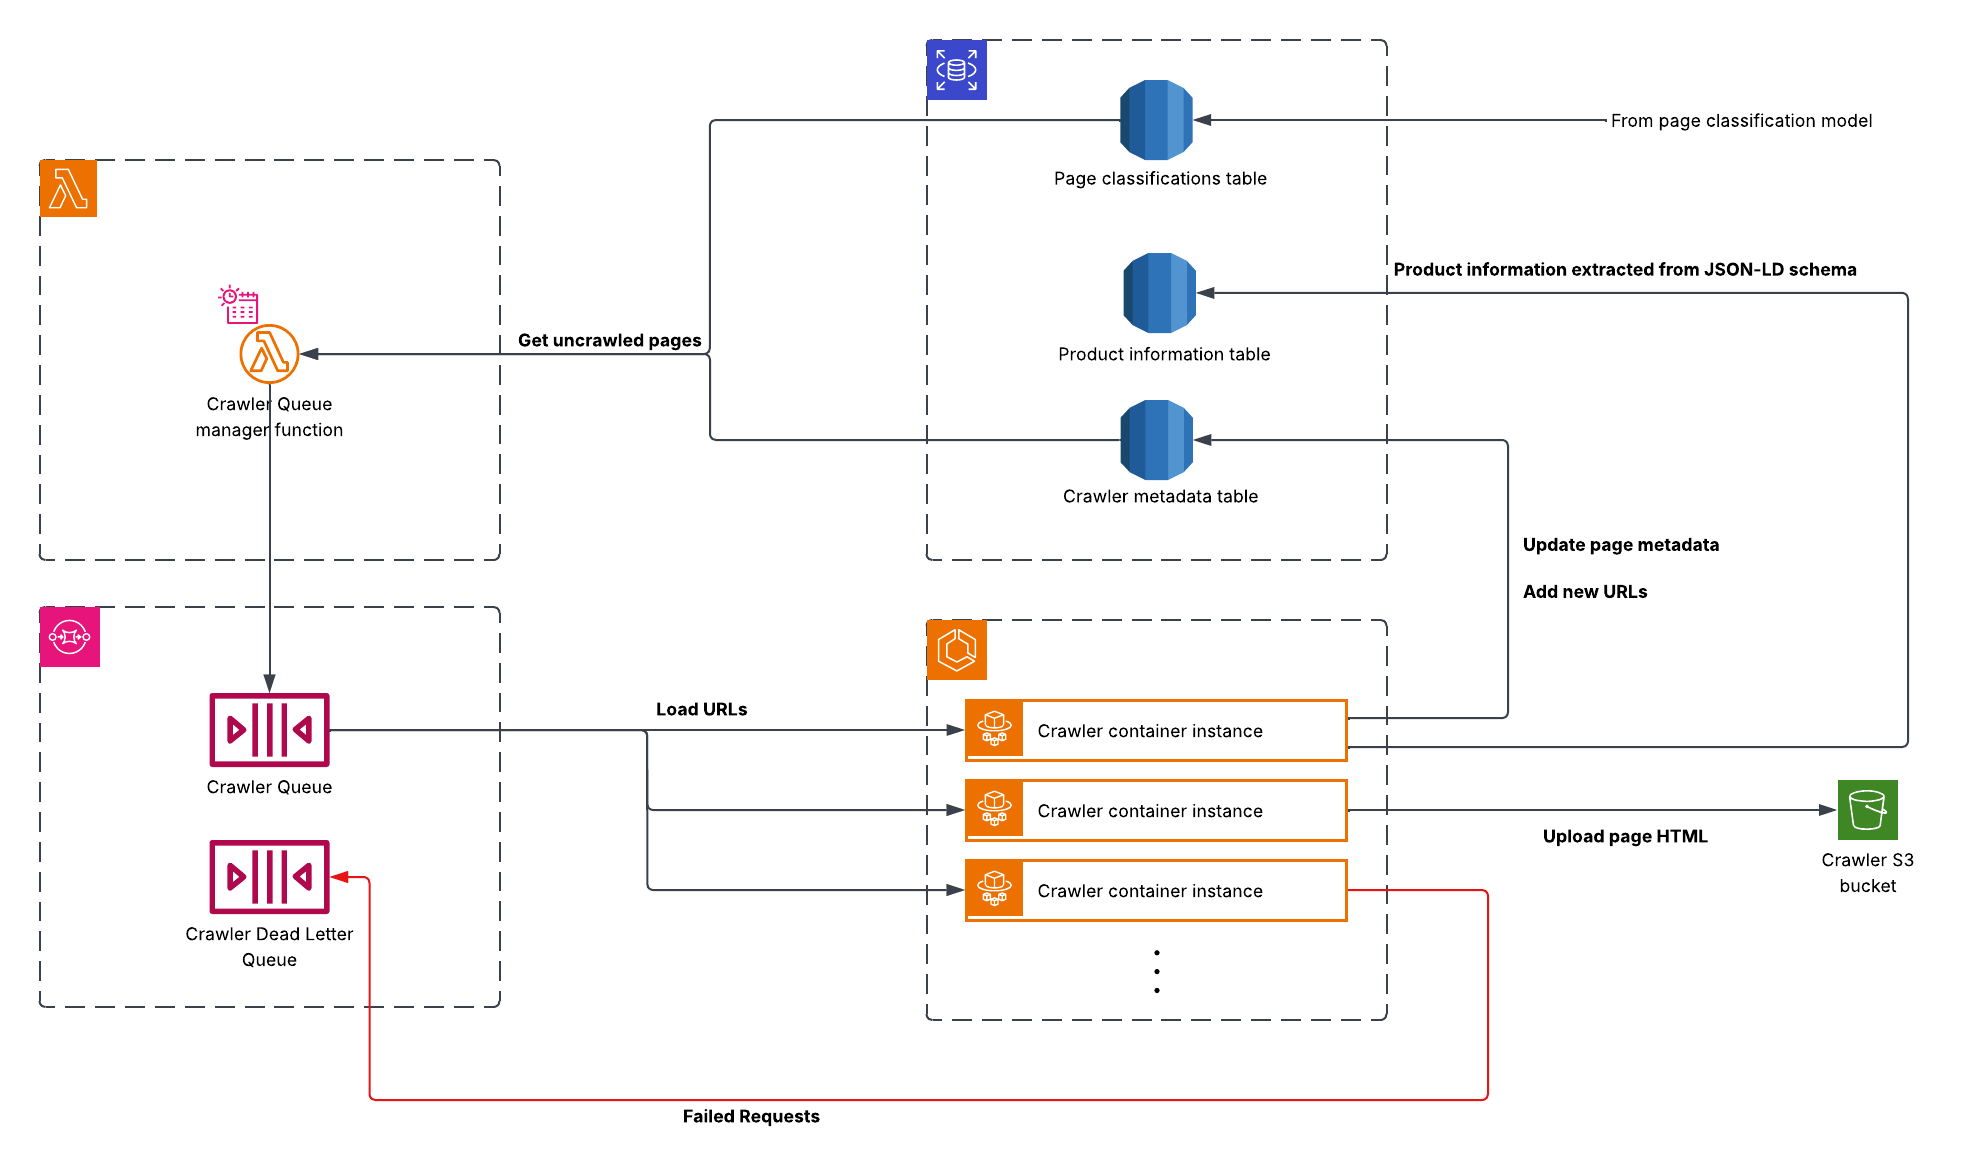
\includegraphics[width=\textwidth]{images/crawler_architecture}~\caption{Distributed crawler system architecture}\label{fig:crawler_system_architecture}
\end{figure}